%
% $XORP: xorp/docs/mld6igmp/mld6igmp_arch.tex,v 1.18 2006/07/05 03:06:28 pavlin Exp $
%

\documentclass[11pt]{article}

%\usepackage[dvips]{changebar}

\usepackage{subfigure}
\usepackage{fullpage}
\usepackage{setspace}
\usepackage{times}
\usepackage{latexsym}
\usepackage{epsfig}
\usepackage{graphicx}
\usepackage{xspace}
\usepackage{color}
\usepackage{amsmath}
%\usepackage[dvipdf]{graphics}
%\usepackage[dvips]{graphicx}
%\usepackage{xorp}

\definecolor{gray}{rgb}{0.5,0.5,0.5}
\newcommand{\etc}{\emph{etc.}\xspace}
\newcommand{\ie}{\emph{i.e.,}\xspace}
\newcommand{\eg}{\emph{e.g.,}\xspace}
%\newcommand{\comment}[1]{{\color{gray}[\textsf{#1}]}}
\newcommand{\comment}[1]{}

% Changebar stuff
% \newenvironment{colorcode}{\color{blue}}{}
% \renewcommand{\cbstart}{\begin{colorcode}}
% \renewcommand{\cbend}{\end{colorcode}}

% \pagestyle{empty}

\begin{document}

\title{XORP MLD/IGMP Daemon \\
\vspace{1ex}
Version 1.2}
\author{ XORP Project					\\
	 International Computer Science Institute	\\
	 Berkeley, CA 94704, USA			\\
         {\it http://www.xorp.org/}			\\
	 {\it feedback@xorp.org}
}
\date{March 8, 2006}

\maketitle

\thispagestyle{empty}


%%%%%%%%%%%%%%%%%%%%%%%%%%%%%%%%%%%%%%%%%%%%%%%%%%%%%%%%%%%%%%%%%%%%%%%
\section{Introduction}


%%%%%%%%%%%%%%%%%%%%%%%%%%%%%%%%%%%%%%%%%%%
\subsection{Overview}

This document provides an overview of the
XORP MLD/IGMP~\cite{MLD-V1,MLD-V2,IGMP-V1,IGMP-V2,IGMP-V3}
Routing Daemon. It is intended to provide a starting point for software
developers who wish to modify this software.

A router running MLD/IGMP interacts with other MLD/IGMP routers and
multicast group members, and keeps state with information about local
multicast membership.

The chosen architecture for the XORP MLD/IGMP implementation emphasizes on
correctness and extensibility rather than high performance or minimal
memory footprint. Typically, the amount of state kept by MLD/IGMP is
relatively small. Further, the multicast routing performance does not
depend on the MLD/IGMP performance, therefore it is not necessary to
optimize the implementation. Only if it turns out that there are
performance issues with MLD/IGMP, we would try to optimize those parts of the
implementation that should prove to be a bottleneck.

The MLD and IGMP implementation is based on the specification in the
 following documents:

\begin{itemize}
  \item{\bf RFC 2236}: Internet Group Management Protocol, Version 2
  \item{\bf RFC 3376}: Internet Group Management Protocol, Version 3
  \item{\bf RFC 2710}: Multicast Listener Discovery (MLD) for IPv6
  \item{\bf RFC 3810}: Multicast Listener Discovery Version 2 (MLDv2) for IPv6
\end{itemize}


%%%%%%%%%%%%%%%%%%%%%%%%%%%%%%%%%%%%%%%%%%%
\subsection{Acronyms}

Acronyms used in this document:

\begin{itemize}

  \item {\bf MFEA}: {\bf M}ulticast {\bf F}orwarding {\bf E}ngine
  {\bf A}bstraction

  \item {\bf MLD/IGMP}: {\bf M}ulticast {\bf L}istener {\bf D}iscovery/{\bf
  I}nternet {\bf G}roup {\bf M}anagement {\bf P}rotocol

  \item {\bf PIM-SM}: {\bf P}rotocol {\bf I}ndependent {\bf M}ulticast--{\bf
  S}parse {\bf M}ode

\end{itemize}


%%%%%%%%%%%%%%%%%%%%%%%%%%%%%%%%%%%%%%%%%%%
\subsection{MLD/IGMP Design Architecture Overview}

\begin{figure}[htbp]
  \begin{center}
    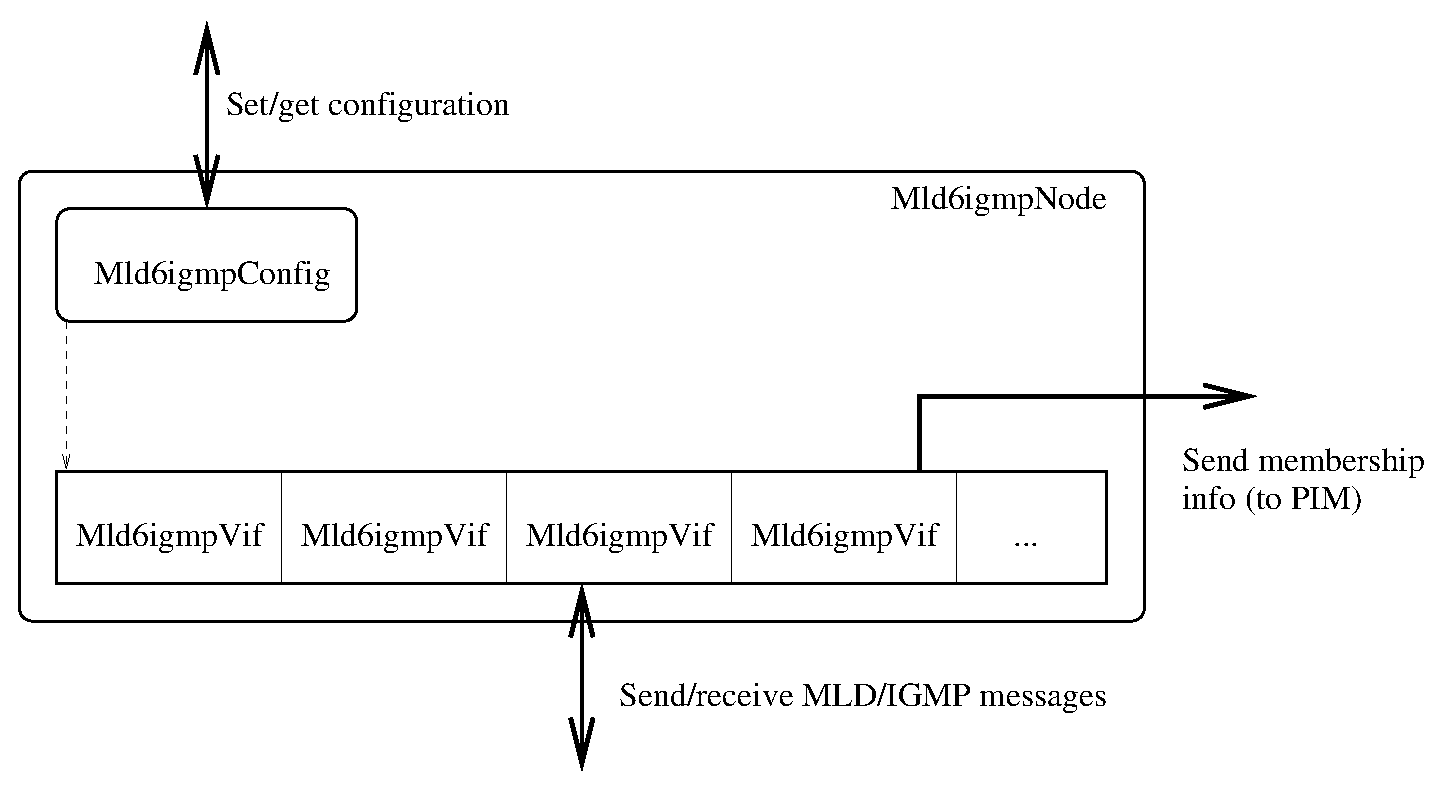
\includegraphics[scale=0.7]{figs/mld6igmp_design_overview}
    \caption{MLD/IGMP design overview}
    \label{fig:mld6igmp_design_overview}
  \end{center}
\end{figure}

Figure~\ref{fig:mld6igmp_design_overview} provides a general overview of the
MLD/IGMP components. For each component there is a C++ class with exactly
the same name. The main components are briefly described below:

\begin{itemize}

  \item {\bf Mld6igmpNode:} a representation of a single MLD/IGMP routing unit
  (\eg a virtual MLD/IGMP router).
  Typically, there would be a single Mld6igmpNode per multicast router.

  \item {\bf Mld6igmpVif:} MLD/IGMP-specific virtual (network) interface that
  is used for sending and receiving MLD/IGMP control packets.

  \item {\bf Mld6igmpConfig:} contains MLD/IGMP-specific configuration.

\end{itemize}

Those components are described in details in
Section~\ref{sec:components_description}.
For information about the interaction between the MLD/IGMP and other modules
see \cite{xorp:multicast_arch}.

%%%%%%%%%%%%%%%%%%%%%%%%%%%%%%%%%%%%%%%%%%%%%%%%%%%%%%%%%%%%%%%%%%%%%%%
\section{Components Description}
\label{sec:components_description}


%%%%%%%%%%%%%%%%%%%%%%%%%%%%%%%%%%%%%%%%%%%
\subsection{Mld6igmpNode Description}

Mld6igmpNode is a representation of a single MLD/IGMP routing unit (\eg a
virtual MLD/IGMP router).
Typically, there would be a single Mld6igmpNode per multicast router.
However, in some cases a multicast router may have more than one
routing unit. For example, it could have one Mld6igmpNode for IPv4, and
another one for IPv6 multicast routing. Further, if we want to
run MLD/IGMP in a simulation environment, each multicast router within that
simulation will be represented by a single Mld6igmpNode.

From a developer's point of view, Mld6igmpNode contains all the state
related to the MLD/IGMP routing unit, and exports the front-end interface
to interact with that unit.
For example, Mld6igmpNode contains the methods to
start/stop or configure MLD/IGMP, or to send/receive MLD/IGMP control packets
to/from the routing unit. Those methods are described in the following files:

\begin{itemize}
  \item \verb=mld6igmp/mld6igmp_node.hh=
  \item \verb=libproto/proto_node.hh=
  \item \verb=libproto/proto_unit.hh=
\end{itemize}

Mld6igmpNode itself does not implement the mechanisms to communicate with
other routing units (\eg to send or receive control packets to/from the
network), or to perform other MLD/IGMP-independent operations such as
joining a multicast routing group. Those mechanisms are outside the scope of
Mld6igmpNode, and must be implemented separately.

Mld6igmpNode contains several pure virtual methods (\eg
\verb=join_multicast_group()= is used to join a multicast group on
an interface) that must be implemented by a class that inherits Mld6igmpNode.
For example, XrlMld6igmpNode is a class that uses Mld6igmpNode as a base
class; XrlMld6igmpNode uses XRL-based communication mechanisms between
Mld6igmpNode and other XORP components such as the MFEA and PIM modules.

By default, Mld6igmpNode is disabled; therefore, on startup it must be
enabled explicitly.

%%%%%%%%%%%%%%%%%%%%%%%%%%%%%%%%%%%%%%%%%%%
\subsection{Mld6igmpVif Description}

Mld6igmpVif is a MLD/IGMP-specific virtual (network) interface that is
used for sending and receiving MLD/IGMP control packets. It includes the
methods for processing and composing MLD/IGMP control messages, as well
as various state per interface (\eg the multicast group membership on an
interface). It contains various state per interface ((\eg the multicast
group membership on an interface), as well as the methods for processing
and composing MLD/IGMP control messages.

Typically, there would be one Mld6igmpVif per network interface
such as physical interface, tunnel, or the loopback
interface. Not all virtual interfaces are
used by MLD/IGMP; for example, all interfaces that are not multicast
capable, and the loopback interface are ignored for multicast
routing.

Typically, from developer's point of view, all interaction with Mld6igmpNode
would be through Mld6igmpNode~\footnote{For simplicity, currently
(March 2006) there are few occasions when XrlMld6igmpNode uses
direct access to Mld6igmpVif.}.

The public interface for Mld6igmpVif contains the methods to manipulate a
virtual (network) interface. Those methods are to start/stop/enable/disable a
virtual interface, and to configure it. The methods are described in
the following files:

\begin{itemize}
  \item \verb=mld6igmp/mld6igmp_vif.hh=
  \item \verb=libxorp/vif.hh=
  \item \verb=libproto/proto_unit.hh=
\end{itemize}

Mld6igmpVif contains state such as group membership information about
local members (a set of objects of class Mld6igmpGroupRecord that contains
sets of objects of class Mld6igmpSourceRecord), and information
about the current MLD/IGMP querier. Also, all 
the MLD/IGMP-specific methods for parsing or constructing MLD/IGMP control
messages when a MLD/IGMP packet is received or sent are implemented as
methods in Mld6igmpVif. The parsing or construction of each message type is
implemented in file \verb=mld6igmp_proto.cc=.

By default, each Mld6igmpVif is disabled; therefore, on startup it must
be enabled explicitly.


%%%%%%%%%%%%%%%%%%%%%%%%%%%%%%%%%%%%%%%%%%%
\subsection{Mld6igmpConfig Description}

Mld6igmpConfig handles the MLD/IGMP-specific
configuration~\footnote{Currently (March 2006), Mld6igmpConfig is not
implemented; rather, all state is kept inside Mld6igmpNode instead.}. This
configuration is used to configure the following units:

\begin{itemize}

  \item Mld6igmpVif: protocol version, membership query related options
  and timer values, etc.

\end{itemize}


%%%%%%%%%%%%%%%%%%%%%%%%%%%%%%%%%%%%%%%%%%%%%%%%%%%%%%%%%%%%%%%%%%%%%%%
%     APPENDIX
%%%%%%%%%%%%%%%%%%%%%%%%%%%%%%%%%%%%%%%%%%%%%%%%%%%%%%%%%%%%%%%%%%%%%%%
\appendix
\section{Modification History}

\begin{itemize}

  \item December 11, 2002: Version 0.1 completed.

  \item March 10, 2003: Updated to match XORP version 0.2 release code;
  cleanup.

  \item June 9, 2003: Bump-up the version to 0.3, and the date.

  \item August 28, 2003: Bump-up the version to 0.4, and the date.

  \item November 6, 2003: Bump-up the version to 0.5, and the date.

  \item July 8, 2004: Bump-up the version to 1.0, and the date.

  \item April 13, 2005: Bump-up the version to 1.1, and the date.

  \item March 8, 2006: Bump-up the version to 1.2, and the date.

  \item July 4, 2006 Updated to include information about the IGMPv3/MLDv2
  implementation.

\end{itemize}


%%%%%%%%%%%%%%%%%%%%%%%%%%%%%%%%%%%%%%%%%%%%%%%%%%%%%%%%%%%%%%%%%%%%%%%
%     BIBLIOGRAPHY
%%%%%%%%%%%%%%%%%%%%%%%%%%%%%%%%%%%%%%%%%%%%%%%%%%%%%%%%%%%%%%%%%%%%%%%
\bibliography{../tex/xorp}
\bibliographystyle{plain}

%%%%%%%%%%%%%%%%%%%%%%%%%%%%%%%%%%%%%%%%%%%%%%%%%%%%%%%%%%%%%%%%%%%%%%%
\end{document}
